\documentclass[a4paper, 12pt, twoside]{article}
\usepackage[utf8]{inputenc}
\usepackage[T1]{fontenc}
\usepackage[francais]{babel}
\usepackage{lmodern}
\usepackage{ae,aecompl}
\usepackage[top=2.5cm, bottom=2cm, left=3cm, right=2.5cm, headheight=15pt]{geometry}
\usepackage{graphicx}
\usepackage{eso-pic}
\usepackage{array}
\usepackage{hyperref}
\usepackage{float}
\input{pagedegarde}

\title{MoodTune -- Générateur de playlist par intelligence artificielle}
\entreprise{Dépôt GitHub : \url{https://github.com/amine95-cloud/moodtune}}
\datedebut{janvier 2026}
\datefin{mai 2026}

\membrea{Sibille Amine 45017331}
\membreb{Larbi Nawfel 45018755}
\membrec{Fourar Anthony 44014695}
\membred{}
\membree{}

\begin{document}

\pagedegarde

\section*{Remerciements}

Nous tenons à remercier nos enseignants de l'Université Paris Nanterre pour leur encadrement tout au long de ce projet, ainsi qu'Anthropic pour la mise à disposition de l'API Claude.

\newpage

\tableofcontents
\newpage

\section{Introduction}

Dans le cadre de notre projet de L1 MIASHS, nous avons développé une application web interactive appelée MoodTune. L'objectif est de concevoir une application utilisant l'intelligence artificielle pour générer des recommandations musicales personnalisées en fonction de l'humeur de l'utilisateur.

L'idée est simple : l'utilisateur décrit en quelques mots comment il se sent, et l'application analyse ce texte grâce à l'API Claude d'Anthropic pour produire une playlist de 8 titres musicaux adaptés à son état émotionnel, accompagnée d'un conseil bien-être et d'une ambiance visuelle dynamique.

Ce projet mobilise plusieurs compétences : programmation web (JavaScript, React), appel à des APIs externes, traitement de données au format JSON et conception d'interfaces utilisateur. L'intelligence artificielle est au cœur du projet, aussi bien pour la génération du code que pour les fonctionnalités de l'application.

Le lien vers le dépôt GitHub est disponible sur la page de garde.

\section{Environnement de travail}

\subsection{Matériel}

Le projet a été développé sur des ordinateurs personnels sous Windows et Linux.
Aucun serveur dédié n'a été nécessaire, l'application fonctionnant entièrement dans le navigateur.

\subsection{Logiciels et outils}

\begin{itemize}
    \item Visual Studio Code : éditeur de code principal.
    \item Git et GitHub : gestion de version et hébergement du code source.
    \item Node.js / npm : environnement d'exécution JavaScript pour React.
    \item Navigateur web : Chrome et Firefox pour tester l'application.
    \item Claude : assistant IA utilisé tout au long du projet.
\end{itemize}

\subsection{Organisation du travail}

Le travail a été réparti via GitHub. Chaque membre a travaillé sur une branche distincte avant de fusionner les modifications. Des échanges réguliers ont permis de synchroniser l'avancement.

\section{Description du projet et objectifs}

\subsection{Présentation générale}

MoodTune est une application web monopage développée en React. Elle permet à un utilisateur de saisir une description de son humeur et reçoit en retour une playlist musicale générée par IA.

L'application repose sur l'API Claude d'Anthropic. Une requête structurée contenant la description de l'humeur est envoyée à l'API, qui renvoie un objet JSON contenant la playlist, des métadonnées sur l'humeur détectée et un conseil bien-être.

\subsection{Fonctionnalités prévues}

\begin{itemize}
    \item Saisie libre de l'humeur par l'utilisateur.
    \item Analyse de l'humeur par l'API Claude.
    \item Génération d'une playlist de 8 titres.
    \item Affichage d'un conseil bien-être personnalisé.
    \item Interface qui change de couleurs dynamiquement selon l'humeur détectée.
    \item Animation d'apparition des titres en cascade.
    \item Bouton de réinitialisation pour générer une nouvelle playlist.
\end{itemize}

\subsection{Objectifs pédagogiques}

Ce projet nous a permis de :

\begin{itemize}
    \item apprendre à utiliser une API externe ;
    \item découvrir le framework React ;
    \item comprendre comment intégrer l'IA dans une application concrète ;
    \item pratiquer la conception d'interfaces utilisateur modernes.
\end{itemize}

\section{Bibliothèques, outils et technologies}

\subsection{React}

React est une bibliothèque JavaScript développée par Meta, permettant de construire des interfaces à partir de composants réutilisables. Nous l'avons utilisé pour structurer l'application en composants indépendants : MoodTune, TrackCard et LoadingBars.

\subsection{API Claude}

L'API Claude est le cœur de notre application. Elle est appelée via une requête fetch en JavaScript. La réponse est un objet JSON contenant la playlist.

Voici un extrait simplifié de l'appel API :

\begin{verbatim}
const res = await fetch("https://api.anthropic.com/v1/messages", {
  method: "POST",
  headers: {
    "Content-Type": "application/json",
    "anthropic-dangerous-direct-browser-access": "true",
  },
  body: JSON.stringify({
    model: "claude-sonnet-4-20250514",
    max_tokens: 1000,
    messages: [{ role: "user", content: prompt }],
  }),
});
const data = await res.json();
\end{verbatim}

\subsection{Google Fonts}

Deux polices de caractères sont importées depuis Google Fonts :

\begin{itemize}
    \item Playfair Display : pour les titres et éléments décoratifs.
    \item DM Sans : pour le texte courant.
\end{itemize}

\subsection{CSS-in-JS}

Les styles sont écrits directement en JavaScript sous forme d'objets, ce qui permet de les rendre dynamiques en fonction de l'humeur détectée.

\section{Travail réalisé}

\subsection{Fonctionnalités réalisées}

Toutes les fonctionnalités prévues ont été implémentées avec succès :

\begin{itemize}
    \item Détection d'humeur en temps réel.
    \item Appel à l'API Claude.
    \item Affichage de la playlist.
    \item Interface dynamique.
\end{itemize}

\subsection{Fonctionnalités non réalisées}

\begin{itemize}
    \item Lecture audio : l'intégration de l'API Spotify a été abandonnée en raison de la complexité de l'authentification OAuth et du temps limité.
    \item Sauvegarde des playlists : cette fonctionnalité avait été envisagée mais n'a pas été implémentée.
\end{itemize}

\subsection{Répartition du travail}

\begin{table}[H]
\centering
\begin{tabular}{|p{4cm}|p{9cm}|}
\hline
\textbf{Membre} & \textbf{Tâches réalisées} \\
\hline
Sibille Amine & Développement du composant principal, intégration de l'API Claude, gestion des états React. \\
\hline
Larbi Nawfel & Design de l'interface, système de thèmes dynamiques, animations. \\
\hline
Fourar Anthony & Rédaction du rapport, tests et débogage, déploiement GitHub. \\
\hline
\end{tabular}
\caption{Répartition réelle du travail entre les membres du groupe}
\end{table}

\section{Difficultés rencontrées}

\subsection{Appel à l'API depuis le navigateur}

La principale difficulté technique a été de faire fonctionner les appels à l'API Claude depuis le navigateur. Par défaut, les navigateurs bloquent ces requêtes avec la politique CORS.

\subsection{Parsing du JSON}

L'API renvoie parfois sa réponse avec des balises Markdown. Nous avons dû nettoyer la réponse avant de la parser :

\begin{verbatim}
const clean = raw.replace(/```json|```/g, "").trim();
const parsed = JSON.parse(clean);
\end{verbatim}

\subsection{Gestion des thèmes dynamiques}

Maintenir la lisibilité du texte sur tous les fonds de couleur a nécessité plusieurs itérations. Nous avons défini 8 palettes complètes pour garantir le contraste.

\subsection{Utilisation de l'IA dans le développement}

Formuler des prompts précis pour obtenir exactement le format JSON souhaité a demandé plusieurs essais. Nous avons appris qu'un prompt structuré avec un exemple de format attendu donne de meilleurs résultats.

\section{Bilan}

\subsection{Conclusion}

Ce projet nous a permis de développer une application web complète en intégrant pour la première fois une intelligence artificielle. MoodTune remplit son objectif : analyser une humeur exprimée en langage naturel et générer une playlist musicale personnalisée.

Au-delà des compétences techniques, ce projet nous a appris à travailler en équipe avec Git, à décomposer un problème complexe et à utiliser l'IA comme outil de développement.

\subsection{Perspectives}

\begin{itemize}
    \item Intégration de l'API Spotify.
    \item Historique des playlists générées.
    \item Analyse d'image pour détecter l'humeur automatiquement.
    \item Version mobile native avec React Native.
\end{itemize}

\newpage

\section{Bibliographie}

\renewcommand{\bibname}{}
\renewcommand{\refname}{}

\begin{thebibliography}{2}
   \bibitem[REACT]{react} Meta Platforms, React -- A JavaScript library for building user interfaces, 2024.
   \bibitem[LAM94]{lam1} L. Lamport, \textit{\LaTeX : A Document Preparation System}, Addison-Wesley, 1994.
\end{thebibliography}

\newpage

\section{Webographie}

\begin{thebibliography}{3}
   \bibitem[ANTH]{anthropic} \url{https://docs.anthropic.com} -- Documentation officielle de l'API Claude, Anthropic, 2025.
   \bibitem[REACTW]{reactweb} \url{https://react.dev} -- Documentation officielle de React, Meta, 2025.
   \bibitem[GH]{github} \url{https://github.com} -- Plateforme de gestion de version.
\end{thebibliography}

\newpage

\section{Annexes}
\appendix
\makeatletter
\def\@seccntformat#1{Annexe~\csname the#1\endcsname:\quad}
\makeatother

\section{Cahier des charges}

\subsection*{Objectif}

Développer une application web utilisant l'IA pour générer des playlists musicales personnalisées selon l'humeur de l'utilisateur.

\subsection*{Contraintes techniques}

\begin{itemize}
    \item Utilisation obligatoire de l'IA.
    \item Interface web accessible depuis un navigateur.
    \item Code source hébergé sur GitHub.
    \item Rapport rédigé avec le template LaTeX fourni.
\end{itemize}

\subsection*{Livrables}

\begin{itemize}
    \item Code source complet sur GitHub.
    \item Application fonctionnelle.
    \item Rapport de projet au format PDF.
\end{itemize}

\section{Exemple d'exécution du projet}

Les captures d'écran ci-dessous illustrent les 4 étapes d'utilisation de MoodTune avec l'humeur ``content''.

\subsection*{Étape 1 -- Page d'accueil}

L'utilisateur arrive sur l'interface avec un fond sombre par défaut et un champ de texte vide.

\begin{figure}[H]
\centering
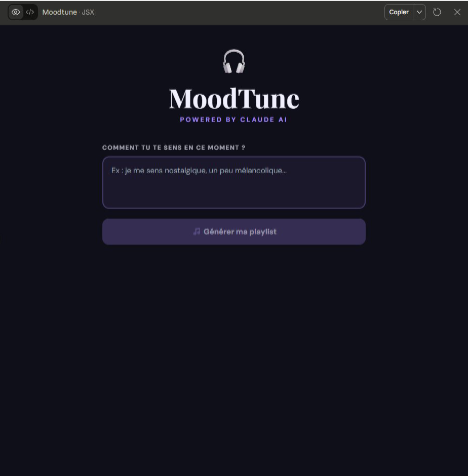
\includegraphics[width=0.7\textwidth]{image1.png}
\caption{Page d'accueil de MoodTune -- thème sombre par défaut}
\end{figure}

\subsection*{Étape 2 -- Saisie de l'humeur}

L'utilisateur tape ``content'' dans le champ. L'interface change immédiatement de couleur : fond jaune ensoleillé, bouton orange.


\begin{figure}[H]
\centering
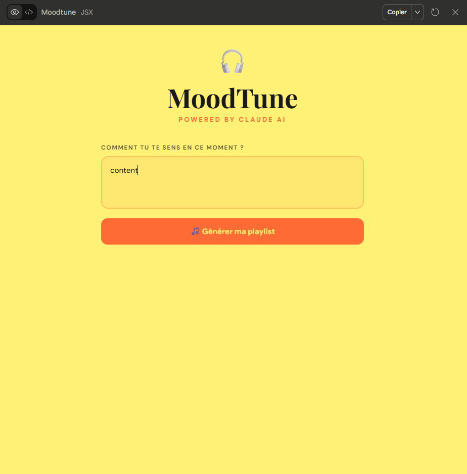
\includegraphics[width=0.7\textwidth]{image2.png}
\caption{Saisie de l'humeur -- le thème change dynamiquement en temps réel}
\end{figure}

\subsection*{Étape 3 -- Résultat : carte d'humeur et début de playlist}

Après génération, l'IA affiche le label ``Joyeux et léger'', une description poétique, le tempo, la couleur émotionnelle et un conseil bien-être.


\begin{figure}[H]
\centering
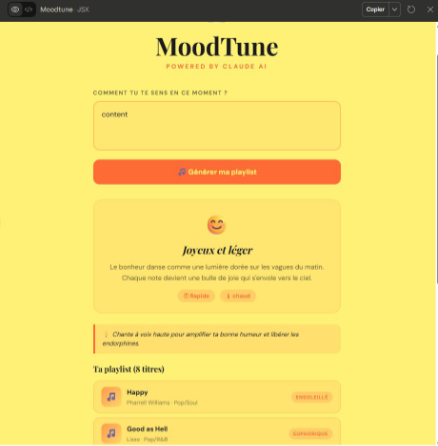
\includegraphics[width=0.7\textwidth]{image3.png}
\caption{Résultat généré par l'application}
\end{figure}

\subsection*{Étape 4 -- Playlist complète}

Les 8 titres s'affichent avec leur artiste, genre et ambiance. Un bouton ``Nouvelle humeur'' permet de recommencer.

\begin{figure}[H]
\centering
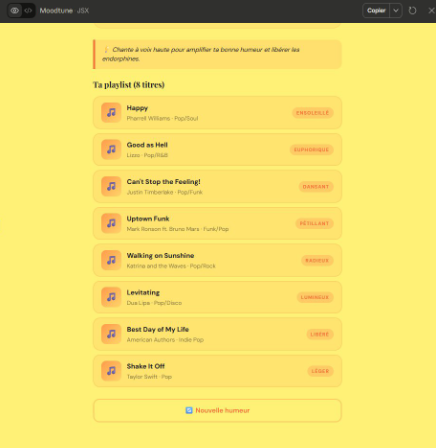
\includegraphics[width=0.7\textwidth]{image4.png}
\caption{Playlist complète générée par MoodTune}
\end{figure}

\section{Manuel utilisateur}

\subsection*{Prérequis}

\begin{itemize}
    \item Un navigateur web moderne.
    \item Une connexion Internet.
\end{itemize}

\subsection*{Utilisation}

\begin{enumerate}
    \item Ouvrir l'application dans le navigateur.
    \item Décrire son humeur dans le champ de texte.
    \item Appuyer sur Entrée ou cliquer sur ``Générer ma playlist''.
    \item Patienter quelques secondes pendant la génération.
    \item Consulter la playlist et le conseil bien-être.
    \item Cliquer sur ``Nouvelle humeur'' pour recommencer.
\end{enumerate}

\subsection*{Remarques}

\begin{itemize}
    \item Plus la description est précise, plus la playlist sera pertinente.
    \item L'interface change de couleur automatiquement selon les mots-clés détectés.
    \item Les titres musicaux sont des suggestions de l'IA, non liées à un service de streaming.
\end{itemize}
\newpage
\section*{Mot de fin}

Nous espérons que ce projet vous aura plu et vous remercions pour votre lecture.

Au revoir et merci.
\end{document}